\documentclass{article}
\usepackage[en]{homework}

\usepackage{float}
\usepackage{pgfplots}
\pgfplotsset{compat=1.15}
\usepackage{mathrsfs}
\usetikzlibrary{arrows}
\definecolor{ffqqqq}{rgb}{1.,0.,0.}
\definecolor{qqwuqq}{rgb}{0.,0.39215686274509803,0.}

\config{Physics\,-\,0}{2026 Spring}{2}

\begin{document}

\begin{problem}
    (20 pts) Consider a Ferris wheel with radius \( R \) rotating at a constant angular velocity \( \omega \).
    \begin{enumerate}[label=(\alph*)]
        \item (10pts) Find the weight you experience at the top and at the bottom of the Ferris wheel.
        \item (5pts) Find the angular velocity for which you would feel weightless.
        \item (5pts) To get some intuition for this number consider one of the largest Ferris wheels in the world, the Star of Nanchang (南昌之星) in Jiangxi province, which has a radius of \( R = 80 \, \text{m} \). Assuming your weight is \( 70 \, \text{kg} \), what is the angular velocity and the period for which you would feel weightless? For comparison, the actual period of the Star of Nanchang is 30 minutes.
    \end{enumerate}
\end{problem}

\begin{solution}
    Suppose the person has mass \( m \). Denote the support force experienced by the person at the top and the bottom of the Ferris wheel as \( N_{\text{t}} \) and \( N_{\text{b}} \) respectively. The weight of the person is \( mg \).\par
    (a) The person has an acceleration of \( a = \omega^2 R \) towards the center of the Ferris wheel. At the top, we have
    \[ -N_{\text{t}} + mg = m \omega^2 R \implies N_{\text{t}} = mg - m\omega^2 R . \]
    At the bottom, we have
    \[ N_{\text{b}} - mg = m \omega^2 R \implies N_{\text{b}} = mg+ m\omega^2 R. \]\par
    (b) To feel weightless, the support force at the top must be at most zero, so we have
    \[ mg - m\omega^2 R \leq 0 \implies \omega \ge \sqrt{\frac{g}{R}}. \]\par
    (c) For \( R = 80 \, \text{m} \), we have
    \[ \omega = \sqrt{\frac{g}{R}} = \sqrt{\frac{9.8\,\text{m}/\text{s}^2}{80\,\text{m}}} \approx 0.35 \, \text{rad/s}. \] The period is
    \[ T = \frac{2\pi}{\omega} \approx \frac{2\pi}{0.35\, \text{rad/s}} \approx 18 \, \text{s}. \] 
\end{solution}

\begin{problem}
    (25 pts) Consider a ball falling in some liquid. The liquid exerts a damping force   
whose magnitude is proportional to the squared speed  of the ball, and whose direction is 
opposite to that of the velocity. Here  is the damping constant. This force is known as quadratic drag and it holds for objects moving fast through viscous fluids. Suppose the ball is released from rest and has mass . 
\begin{enumerate}[label=(\alph*)]
    \item (10pts) Draw the vector fields for the gravitational and damping forces.
    \item (10pts) Find the velocity as a function of time.
    \item (5pts) Determine the terminal velocity of the ball when .
\end{enumerate}
\end{problem}

\begin{solution}
    (a) As shown below.
    \begin{figure}[H]
    \centering
    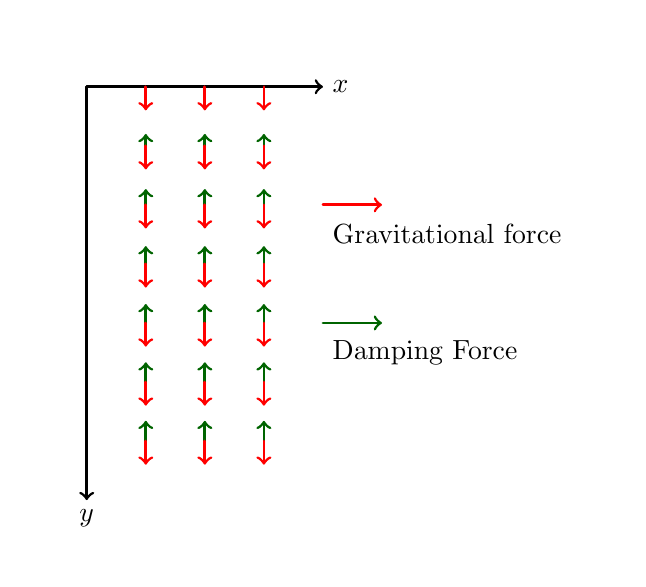
\begin{tikzpicture}[line cap=round,line join=round,x=1.5cm,y=1.5cm]
        \clip(-0.5,-4) rectangle (4.5,0.5);
        \draw [line width=1pt,->] (0.,0.)-- (2.,0.);
        \draw [line width=1pt,->] (0.,0.)-- (0.,-3.5);
        \draw [line width=1pt,->,color=qqwuqq] (0.5,-0.5)-- (0.5,-0.4);
        \draw [line width=1pt,->,color=qqwuqq] (0.5,-1.)-- (0.5,-0.8666666666666667);
        \draw [line width=1pt,->,color=qqwuqq] (0.5,-1.5)-- (0.5,-1.35);
        \draw [line width=1pt,->,color=qqwuqq] (0.5,-2.)-- (0.5,-1.84);
        \draw [line width=1pt,->,color=qqwuqq] (0.5,-2.5)-- (0.5,-2.3333333333333335);
        \draw [line width=1pt,->,color=qqwuqq] (0.5,-3.)-- (0.5,-2.8285714285714287);
        \draw [line width=1pt,->,color=qqwuqq] (1.,-0.5)-- (1.,-0.4);
        \draw [line width=1pt,->,color=qqwuqq] (1.,-1.)-- (1.,-0.8666666666666667);
        \draw [line width=1pt,->,color=qqwuqq] (1.,-1.5)-- (1.,-1.35);
        \draw [line width=1pt,->,color=qqwuqq] (1.,-2.)-- (1.,-1.84);
        \draw [line width=1pt,->,color=qqwuqq] (1.,-2.5)-- (1.,-2.3333333333333335);
        \draw [line width=1pt,->,color=qqwuqq] (1.,-3.)-- (1.,-2.8285714285714287);
        \draw [line width=1pt,->,color=qqwuqq] (1.5,-0.5)-- (1.5,-0.4);
        \draw [line width=1pt,->,color=qqwuqq] (1.5,-1.)-- (1.5,-0.8666666666666667);
        \draw [line width=1pt,->,color=qqwuqq] (1.5,-1.5)-- (1.5,-1.35);
        \draw [line width=1pt,->,color=qqwuqq] (1.5,-2.)-- (1.5,-1.84);
        \draw [line width=1pt,->,color=qqwuqq] (1.5,-2.5)-- (1.5,-2.3333333333333335);
        \draw [line width=1pt,->,color=qqwuqq] (1.5,-3.)-- (1.5,-2.8285714285714287);
        \draw [line width=1pt,->,color=ffqqqq] (0.5,0.)-- (0.5,-0.2);
        \draw [line width=1pt,->,color=ffqqqq] (0.5,-0.5)-- (0.5,-0.7);
        \draw [line width=1pt,->,color=ffqqqq] (0.5,-1.)-- (0.5,-1.2);
        \draw [line width=1pt,->,color=ffqqqq] (0.5,-1.5)-- (0.5,-1.7);
        \draw [line width=1pt,->,color=ffqqqq] (0.5,-2.)-- (0.5,-2.2);
        \draw [line width=1pt,->,color=ffqqqq] (0.5,-2.5)-- (0.5,-2.7);
        \draw [line width=1pt,->,color=ffqqqq] (0.5,-3.)-- (0.5,-3.2);
        \draw [line width=1pt,->,color=ffqqqq] (1.,0.)-- (1.,-0.2);
        \draw [line width=1pt,->,color=ffqqqq] (1.,-0.5)-- (1.,-0.7);
        \draw [line width=1pt,->,color=ffqqqq] (1.,-1.)-- (1.,-1.2);
        \draw [line width=1pt,->,color=ffqqqq] (1.,-1.5)-- (1.,-1.7);
        \draw [line width=1pt,->,color=ffqqqq] (1.,-2.)-- (1.,-2.2);
        \draw [line width=1pt,->,color=ffqqqq] (1.,-2.5)-- (1.,-2.7);
        \draw [line width=1pt,->,color=ffqqqq] (1.,-3.)-- (1.,-3.2);
        \draw [line width=1pt,->,color=ffqqqq] (1.5,0.)-- (1.5,-0.2);
        \draw [line width=1pt,->,color=ffqqqq] (1.5,-0.5)-- (1.5,-0.7);
        \draw [line width=1pt,->,color=ffqqqq] (1.5,-1.)-- (1.5,-1.2);
        \draw [line width=1pt,->,color=ffqqqq] (1.5,-1.5)-- (1.5,-1.7);
        \draw [line width=1pt,->,color=ffqqqq] (1.5,-2.)-- (1.5,-2.2);
        \draw [line width=1pt,->,color=ffqqqq] (1.5,-2.5)-- (1.5,-2.7);
        \draw [line width=1pt,->,color=ffqqqq] (1.5,-3.)-- (1.5,-3.2);
        \draw [line width=1pt,->,color=ffqqqq] (2.,-1.)-- (2.5,-1.);
        \draw [line width=1pt,->,color=qqwuqq] (2.,-2.)-- (2.5,-2.);
        \draw (2,0) node[anchor=west] {$x$};
        \draw (0,-3.5) node[anchor=north] {$y$};
        \draw (2,-1.25) node[anchor=west] {Gravitational force};
        \draw (2,-2.25) node[anchor=west] {Damping Force};
    \end{tikzpicture}
    \end{figure}\par
    (b) Denote the velocity of the ball at time \( t \) as \( v(t) \), with the positive direction being downward. We have
    \[ m \frac{\d v}{\d t} = mg - kv^2\ \implies\ \frac{m\d v}{mg-kv^2}=\d t  \]
    \[ \implies\ \int_{0}^{v(t)}\frac{m\d v}{mg-k v^2}=t\ \implies\ t=\sqrt{\frac{m }{gk}}\,\text{arctanh}\left(\sqrt{\frac{k}{mg}}v(t)\right) \]
    \[ \implies\ v(t)=\sqrt{\frac{mg}{k}}\tanh \left(\sqrt{\frac{gk}{m}}t \right). \]
    (c) Take \( t\to+\infty \) , we got the terminal velocity
    \[ v_{\text{terminal}} = \sqrt{\frac{mg}{k}}. \]
\end{solution}

\begin{problem}
    (20 pts) In the figure below, each of the blocks was weight \( w \). Assuming the pulleys are frictionless and the ropes are massless, draw a diagram of the forces acting on the blocks in each case, and calculate the tension in the rope in terms of \( w \).
\end{problem}

\begin{solution}
    As shown below.
    \begin{figure}[H]
        \centering
        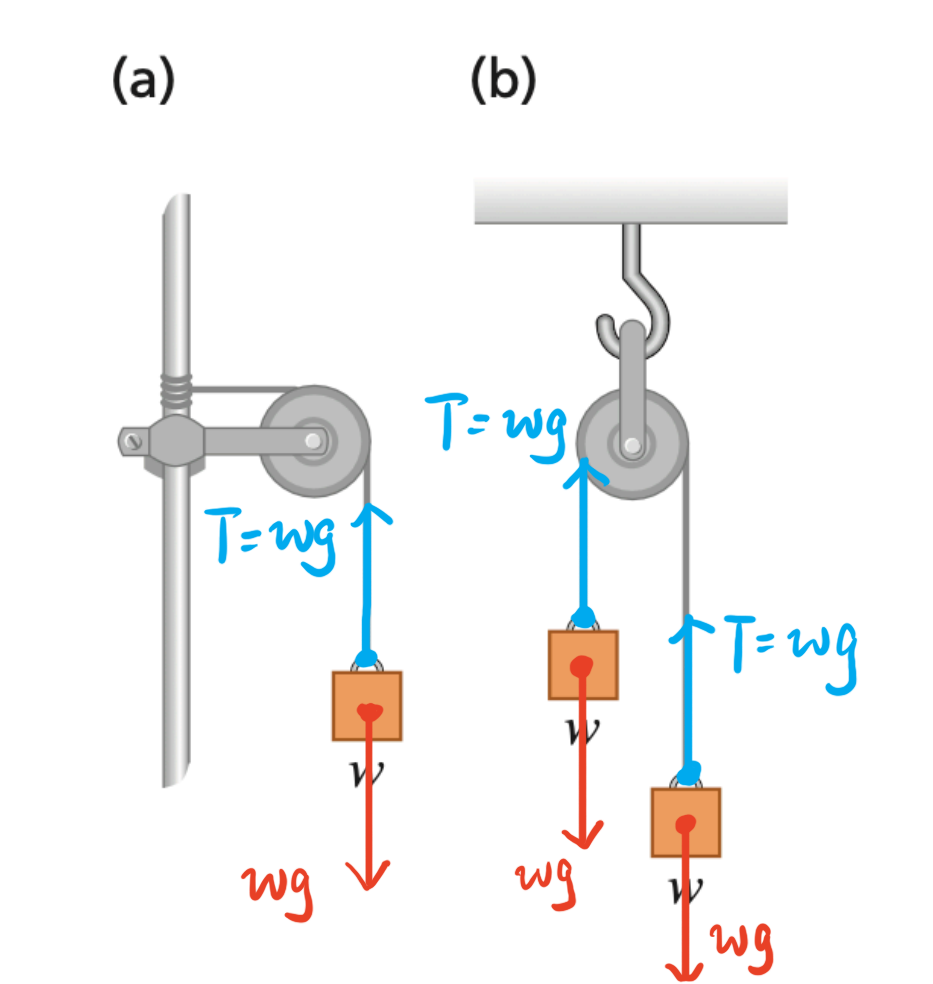
\includegraphics[width=0.4\textwidth]{1.png}
    \end{figure}
\end{solution}

\begin{problem}
    (35 pts) Consider the system illustrated in the figure below where the masses \( m_1 \), \( m_2 \), and \( m_3 \) are arbitrary. Let the system be released from rest. Assuming that the pulleys are frictionless and the ropes are massless, compute the following:
    \begin{enumerate}[label=(\alph*)]
        \item (15 pts) The acceleration of each of the blocks.
        \item (10 pts) The tension in the rope \( A  \) and \( C \).
        \item (10 pts) What happens to answers (a) and (b) when \( m_1=m_2=m \) and \( m_3=2m \)? Is this the expected results?
    \end{enumerate}
    \begin{center}
        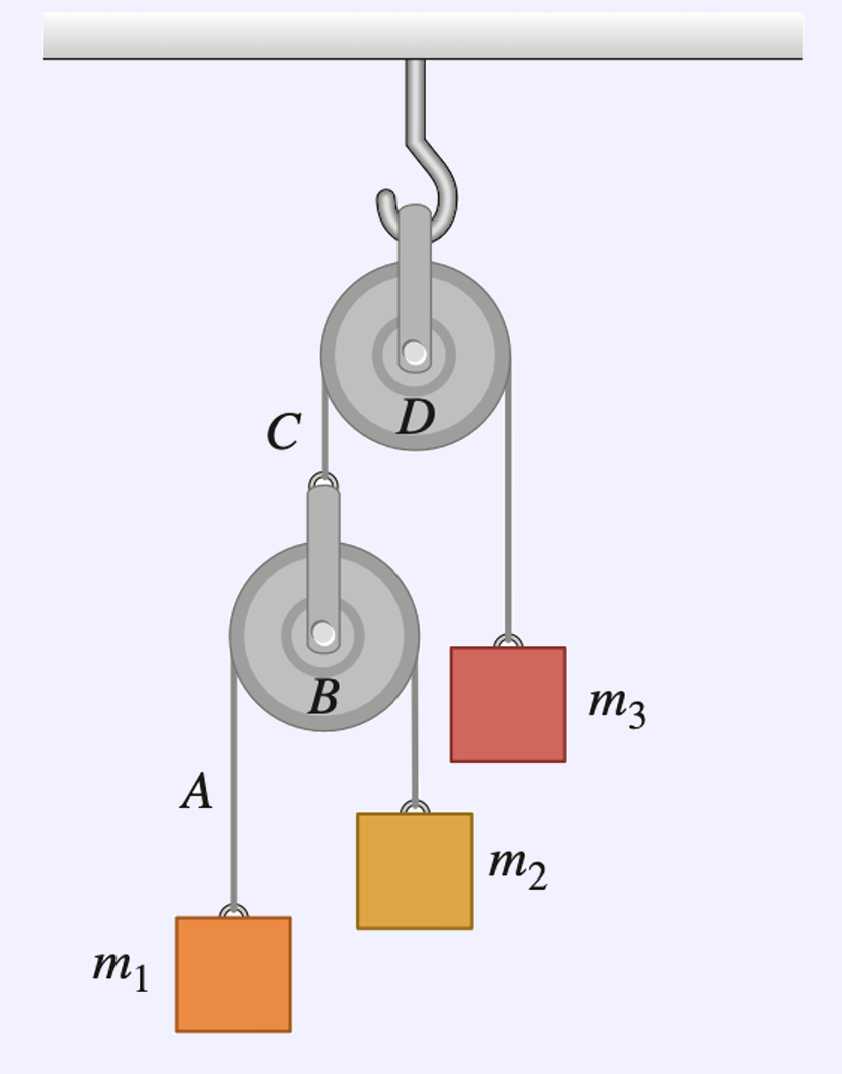
\includegraphics[width=0.4\textwidth]{2.png}
    \end{center}
\end{problem}

\begin{solution}
    (a) and (b) \ \ Denote the distance from the ceiling to \( m_1,\,m_2,\,m_3 \) as \( x_1,\,x_2,\,x_3 \) respectively, and the acceleration of \( m_1,\,m_2,\,m_3 \) as \( a_1,\,a_2,\,a_3 \) respectively, with the positive direction being downward. We immediately got the relation
    \[ a_i=\ddot{x}_i \ (1\le i\le 3),\quad x_1+x_2+2x_3=\text{const.}\implies a_1+a_2+2a_3=0. \tag{1}\] \par
    Denote the tension in rope \( A \) and \( C \) as \( T_\mathrm{A} \) and \( T_\mathrm{C} \) respectively. Since the pulley B is massless, we have \( 2T_\mathrm{A}=T_\mathrm{C} \), hence we can assume that
    \[ T_\mathrm{A }:=T,\quad T_\mathrm{C }:=2T. \tag{2}\] \par
    Consider Newton's second law for each block, we have
    \[ \begin{cases}
        m_1 a_1 &= m_1 g - T_\mathrm{A }, \\
        m_2 a_2 &= m_2 g - T_\mathrm{A }, \\
        m_3 a_3 &= m_3 g - T_\mathrm{C }.
    \end{cases} \]
    Combining with the relation (1) and (2) and solving those equations, we got
    \[ \begin{cases}
        a_1=\dfrac{4m_1m_2+m_1m_3-3m_2m_3}{4m_1m_2+m_1m_3+m_2m_3}g,\\
        a_2=\dfrac{4m_1m_2-3m_1m_3+m_2m_3}{4m_1m_2+m_1m_3+m_2m_3}g,\\
        a_3=\dfrac{-4m_1m_2+m_1m_3+m_2m_3}{4m_1m_2+m_1m_3+m_2m_3}g,\\
        T_\mathrm{A}=\dfrac{4m_1m_2m_3g}{4m_1m_2+m_1m_3+m_2m_3},\\
        T_\mathrm{C}=\dfrac{8m_1m_2m_3g}{4m_1m_2+m_1m_3+m_2m_3}.
    \end{cases} \]  \par
    (c) Take \( m_1=m_2=m \) and \( m_3=2m \), we have
    \[ \begin{cases}
        a_1=a_2=0,\\
        a_3=0,\\
        T_\mathrm{A}=mg,\\
        T_\mathrm{C}=2mg.
    \end{cases} \]  \par
    This is the expected result, as the system is in equilibrium when the masses are given as above.
\end{solution}

\end{document}